\documentclass[12pt,a4paper]{article}
\usepackage{amsmath,amssymb,mathrsfs,tikz,times,pifont}
\usepackage{enumitem}
\newcommand\circitem[1]{%
\tikz[baseline=(char.base)]{
\node[circle,draw=gray, fill=red!55,
minimum size=1.2em,inner sep=0] (char) {#1};}}
\newcommand\boxitem[1]{%
\tikz[baseline=(char.base)]{
\node[fill=cyan,
minimum size=1.2em,inner sep=0] (char) {#1};}}
\setlist[enumerate,1]{label=\protect\circitem{\arabic*}}
\setlist[enumerate,2]{label=\protect\boxitem{\alph*}}
%%%::::::by chnini ameur :::::::%%%
\everymath{\displaystyle}
\usepackage[left=1cm,right=1cm,top=1cm,bottom=1.7cm]{geometry}
\usepackage[colorlinks=true, linkcolor=blue, urlcolor=blue, citecolor=blue]{hyperref}
\usepackage{array,multirow}
\usepackage[most]{tcolorbox}
\usepackage{varwidth}
\usepackage{float} %pour utiliser l'option [H] qui force l'image à apparaître exactement à l'endroit où elle est placée dans le code.
\tcbuselibrary{skins,hooks}
\usetikzlibrary{patterns}
%%%::::::by chnini ameur :::::::%%%
\newtcolorbox{exa}[2][]{enhanced,breakable,before skip=2mm,after skip=5mm,
colback=yellow!20!white,colframe=black!20!blue,boxrule=0.5mm,
attach boxed title to top left ={xshift=0.6cm,yshift*=1mm-\tcboxedtitleheight},
fonttitle=\bfseries,
title={#2},#1,
% varwidth boxed title*=-3cm,
boxed title style={frame code={
\path[fill=tcbcolback!30!black]
([yshift=-1mm,xshift=-1mm]frame.north west)
arc[start angle=0,end angle=180,radius=1mm]
([yshift=-1mm,xshift=1mm]frame.north east)
arc[start angle=180,end angle=0,radius=1mm];
\path[left color=tcbcolback!60!black,right color = tcbcolback!60!black,
middle color = tcbcolback!80!black]
([xshift=-2mm]frame.north west) -- ([xshift=2mm]frame.north east)
[rounded corners=1mm]-- ([xshift=1mm,yshift=-1mm]frame.north east)
-- (frame.south east) -- (frame.south west)
-- ([xshift=-1mm,yshift=-1mm]frame.north west)
[sharp corners]-- cycle;
},interior engine=empty,
},interior style={top color=yellow!5}}
%%%%%%%%%%%%%%%%%%%%%%%

\usepackage{fancyhdr}
\usepackage{eso-pic}         % Pour ajouter des éléments en arrière-plan
% Commande pour ajouter du texte en arrière-plan
\usepackage{tkz-tab}
\AddToShipoutPicture{
    \AtTextCenter{%
        \makebox[0pt]{\rotatebox{80}{\textcolor[gray]{0.5}{\fontsize{5cm}{5cm}\selectfont PGB}}}
    }
}
\usepackage{lastpage}
\fancyhf{}
\pagestyle{fancy}
\renewcommand{\footrulewidth}{1pt}
\renewcommand{\headrulewidth}{0pt}
\renewcommand{\footruleskip}{10pt}
\fancyfoot[R]{
\color{blue}\ding{45}\ \textbf{2025}
}
\fancyfoot[L]{
\color{blue}\ding{45}\ \textbf{Prof:M. BA}
}
\cfoot{\bf
\thepage /
\pageref{LastPage}}
\begin{document}
\renewcommand{\arraystretch}{1.5}
\renewcommand{\arrayrulewidth}{1.2pt}
\begin{tikzpicture}[overlay,remember picture]
\node[draw=blue,line width=1.2pt,fill=purple,text=blue,inner sep=3mm,rounded corners,pattern=dots]at ([yshift=-2.5cm]current page.north) {\begingroup\setlength{\fboxsep}{0pt}\colorbox{white}{\begin{tabular}{|*1{>{\centering \arraybackslash}p{0.28\textwidth}} |*2{>{\centering \arraybackslash}p{0.2\textwidth}|} *1{>{\centering \arraybackslash}p{0.19\textwidth}|} }
\hline
\multicolumn{3}{|c|}{$\diamond$$\diamond$$\diamond$\ \textbf{Lycée de Dindéfélo}\ $\diamond$$\diamond$$\diamond$ }& \textbf{A.S. : 2024/2025} \\ \hline
\textbf{Matière: Mathématiques}& \textbf{Niveau : 2nd}\textbf{L} &\textbf{Date: 14/02/2025} & \textbf{Rendre le 19 à 10H} \\ \hline
\multicolumn{4}{|c|}{\parbox[c]{10cm}{\begin{center}
\textbf{{\Large\sffamily Correction Dm}}
\end{center}}} \\ \hline
\end{tabular}}\endgroup};
\end{tikzpicture}
\vspace{3cm}

\section*{\underline{Exercice 1 :}3pts}
\begin{enumerate}
\item Calculons les expressions suivantes et donnons les résultats sous la forme de fractions irréductibles :
\[
\begin{aligned}
    A &= \left( -1 + \frac{1}{\frac{1}{4} + \frac{1}{2}} \right) \times \left( 1 - \frac{1}{2} \right) \\[6pt]
    &= \left( -1 + \frac{1}{\frac{1}{4} + \frac{2}{4}} \right) \times \left( \frac{1}{2} \right) \\[6pt]
    &= \left( -1 + \frac{1}{\frac{3}{4}} \right) \times \frac{1}{2} \\[6pt]
    &= \left( -1 + \frac{4}{3} \right) \times \frac{1}{2} \\[6pt]
    &= \left( \frac{-3}{3} + \frac{4}{3} \right) \times \frac{1}{2} \\[6pt]
    &= \frac{1}{3} \times \frac{1}{2} \\[6pt]
    &= \frac{1}{6}
\end{aligned}
\]

\[
\begin{aligned}
    A &= \left( -1 + \frac{1}{\frac{1}{1} + \frac{1}{2}} \right) \times \left( 1 - \frac{1}{2} \right) \\[6pt]
    &= \left( -1 + \frac{1}{\frac{1}{4} + \frac{2}{4}} \right) \times \left( \frac{1}{2} \right) \\[6pt]
    &= \left( -1 + \frac{1}{\frac{3}{4}} \right) \times \frac{1}{2} \\[6pt]
    &= \left( -1 + \frac{4}{3} \right) \times \frac{1}{2} \\[6pt]
    &= \left( \frac{-3}{3} + \frac{4}{3} \right) \times \frac{1}{2} \\[6pt]
    &= \frac{1}{3} \times \frac{1}{2} \\[6pt]
    &= \frac{1}{6}
\end{aligned}
\]

\begin{tcolorbox}[colback=yellow!20, colframe=black, sharp corners]
    \[
    \mathbf{A = \frac{1}{6}}\quad\quad     \textbf{0,75pt}
    \]
\end{tcolorbox}

\[
\begin{aligned}
    B &= \left( 1 - \frac{1}{3} \right) \times \left( 3 - \frac{\frac{3}{2}}{1 + \frac{1}{3}} \right) \\[6pt]
    &= \left( \frac{3}{3} - \frac{1}{3} \right) \times \left( 3 - \frac{\frac{3}{2}}{\frac{4}{3}} \right) \\[6pt]
    &= \frac{2}{3} \times \left( 3 - \frac{3}{2} \times \frac{3}{4} \right) \\[6pt]
    &= \frac{2}{3} \times \left( 3 - \frac{9}{8} \right) \\[6pt]
    &= \frac{2}{3} \times \left( \frac{24}{8} - \frac{9}{8} \right) \\[6pt]
    &= \frac{2}{3} \times \frac{15}{8} \\[6pt]
    &= \frac{2 \times 15}{3 \times 8} \\[6pt]
    &= \frac{30}{24} \\[6pt]
    &= \frac{5}{4}
\end{aligned}
\]

\begin{tcolorbox}[colback=yellow!20, colframe=black, sharp corners]
    \[
    \mathbf{B = \frac{5}{4}}\quad\quad     \textbf{0,75pt}
    \]
\end{tcolorbox}

\item Écrivons sous la forme \( a\sqrt{b} \) l’expression suivante :
\[
\begin{aligned}
    E &= 2\sqrt{28} + 2\sqrt{63} + 3\sqrt{7} \\[6pt]
    &= 2 \times \sqrt{4 \times 7} + 2 \times \sqrt{9 \times 7} + 3\sqrt{7} \\[6pt]
    &= 2 \times \sqrt{4} \times \sqrt{7} + 2 \times \sqrt{9} \times \sqrt{7} + 3\sqrt{7} \\[6pt]
    &= 2 \times 2\sqrt{7} + 2 \times 3\sqrt{7} + 3\sqrt{7} \\[6pt]
    &= 4\sqrt{7} + 6\sqrt{7} + 3\sqrt{7} \\[6pt]
    &= (4 + 6 + 3) \sqrt{7} \\[6pt]
    &= 13\sqrt{7}
\end{aligned}
\]

\begin{tcolorbox}[colback=yellow!20, colframe=black, sharp corners]
    \[
    \mathbf{E = 13\sqrt{7}}\quad\quad     \textbf{0,75pt}
    \]
\end{tcolorbox}
\item Écrivons l’expression suivante sous la forme \( 2^m \times 5^n \times 7^p \) :
\[
\begin{aligned}
    A &= \frac{7^5 \times 4^2 \times 5^6}{5^3 \times 7^3 \times 8^3} \\[6pt]
    &= \frac{7^5 \times (2^2)^2 \times 5^6}{5^3 \times 7^3 \times (2^3)^3} \\[6pt]
    &= \frac{7^5 \times 2^4 \times 5^6}{5^3 \times 7^3 \times 2^9} \\[6pt]
    &= 7^{5-3} \times 2^{4-9} \times 5^{6-3} \\[6pt]
    &= 7^2 \times 2^{-5} \times 5^3 \\[6pt]
    &= \frac{5^3 \times 7^2}{2^5}
\end{aligned}
\]

\begin{tcolorbox}[colback=yellow!20, colframe=black, sharp corners]
    \[
    \mathbf{A = \frac{5^3 \times 7^2}{2^5}}\quad\quad     \textbf{0,75pt}
    \]
\end{tcolorbox}

\end{enumerate}

\section*{\underline{Exercice 2: }6pts}
\begin{enumerate}
    \item Mettons les trinômes ci-dessus sous forme canonique 

\[
A = 5x^2 - 7x - 34
\]

\[
\begin{aligned}
a &= 5, & b &= -7, & c &= -34
\end{aligned}
\]

\[
\begin{aligned}
A &= a \left[\left( x - \frac{b}{2a} \right)^2 + \frac{b^2 - 4ac}{4a^2} \right] \\
  &= 5 \left[\left( x - \frac{-7}{2 \times 5} \right)^2 + \frac{(-7)^2 - 4(5)(-34)}{4(5^2)} \right] \\
  &= 5 \left[\left( x - \frac{7}{10} \right)^2 + \frac{49 + 680}{100} \right] \\
  &= 5 \left[\left( x - \frac{7}{10} \right)^2 + \frac{729}{100} \right] \\
  &= 5 \left[\left( x - \frac{7}{10} \right)^2 + \frac{81}{11} \right] \\
  &= 5 \left( x - \frac{7}{10} \right)^2 + \frac{405}{11}
\end{aligned}
\]

\begin{tcolorbox}[colback=yellow!20, colframe=black, sharp corners]
    \[
    \mathbf{A =  5 \left[\left( x - \frac{7}{10} \right)^2 + \frac{81}{11} \right]}\quad\quad     \textbf{0,75pt}
    \]
\end{tcolorbox}

\[
B = 2x^2 - 5x + 3
\]

\[
\begin{aligned}
a &= 2, & b &= -5, & c &= 3
\end{aligned}
\]

\[
\begin{aligned}
B &= a \left[\left( x - \frac{b}{2a} \right)^2 + \frac{b^2 - 4ac}{4a^2} \right] \\
  &= 2 \left[\left( x - \frac{-5}{2 \times 2} \right)^2 + \frac{(-5)^2 - 4(2)(3)}{4(2^2)} \right] \\
  &= 2 \left[\left( x - \frac{5}{4} \right)^2 + \frac{25 - 24}{16} \right] \\
  &= 2 \left[\left( x - \frac{5}{4} \right)^2 + \frac{1}{16} \right] \\
  &= 2 \left( x - \frac{5}{4} \right)^2 + \frac{2}{16} \\
  &= 2 \left( x - \frac{5}{4} \right)^2 + \frac{1}{8}
\end{aligned}
\]

\begin{tcolorbox}[colback=yellow!20, colframe=black, sharp corners]
    \[
    \mathbf{B =  2 \left[\left( x - \frac{5}{4} \right)^2 + \frac{1}{16} \right]}\quad\quad     \textbf{0,75pt}
    \]
\end{tcolorbox}

\[
C = -5x^2 + 9x - 5
\]

\[
\begin{aligned}
a &= -5, & b &= 9, & c &= -5
\end{aligned}
\]

\[
\begin{aligned}
C &= a \left[\left( x - \frac{b}{2a} \right)^2 + \frac{b^2 - 4ac}{4a^2} \right] \\
  &= -5 \left[\left( x - \frac{9}{2 \times (-5)} \right)^2 + \frac{(9)^2 - 4(-5)(-5)}{4(-5)^2} \right] \\
  &= -5 \left[\left( x - \frac{9}{-10} \right)^2 + \frac{81 - 100}{100} \right] \\
  &= -5 \left[\left( x + \frac{9}{10} \right)^2 + \frac{-19}{100} \right] \\
\end{aligned}
\]

\begin{tcolorbox}[colback=yellow!20, colframe=black, sharp corners]
    \[
    \mathbf{C = -5 \left[\left( x + \frac{9}{10} \right)^2 + \frac{-19}{100} \right]}\quad\quad \textbf{0,75pt}
    \]
\end{tcolorbox}

\[
D = 2x^2 - 6x + 5
\]

\[
\begin{aligned}
a &= 2, & b &= -6, & c &= 5
\end{aligned}
\]

\[
\begin{aligned}
D &= a \left[\left( x - \frac{b}{2a} \right)^2 + \frac{b^2 - 4ac}{4a^2} \right] \\
  &= 2 \left[\left( x - \frac{-6}{2 \times 2} \right)^2 + \frac{(-6)^2 - 4(2)(5)}{4(2^2)} \right] \\
  &= 2 \left[\left( x - \frac{6}{4} \right)^2 + \frac{36 - 40}{16} \right] \\
  &= 2 \left[\left( x - \frac{3}{2} \right)^2 + \frac{-4}{16} \right] \\
  &= 2 \left[\left( x - \frac{3}{2} \right)^2 + \frac{-1}{4} \right] \\
\end{aligned}
\]

\begin{tcolorbox}[colback=yellow!20, colframe=black, sharp corners]
    \[
    \mathbf{D = 2 \left[\left( x - \frac{3}{2} \right)^2 + \frac{-1}{4} \right]}\quad\quad \textbf{0,75pt}
    \]
\end{tcolorbox}
\item Factorisons si possible les trinômes

\paragraph{•}  
\(
A = 5x^2 - 7x - 34
\)

\[
\begin{aligned}
\Delta &= b^2 - 4ac \\
       &= (-7)^2 - 4(5)(-34) \\
       &= 49 + 680 \\
       &= 729
\end{aligned}
\]

\[
\begin{aligned}
x_1 &= \frac{-b + \sqrt{\Delta}}{2a} \\
    &= \frac{-(-7) + \sqrt{729}}{2(5)} \\
    &= \frac{7 + 27}{10} \\
    &= \frac{34}{10} \\
    &= \frac{17}{5}
\end{aligned}
\]

\[
\begin{aligned}
x_2 &= \frac{-b - \sqrt{\Delta}}{2a} \\
    &= \frac{-(-7) - \sqrt{729}}{2(5)} \\
    &= \frac{7 - 27}{10} \\
    &= \frac{-20}{10} \\
    &= -2
\end{aligned}
\]

\[
\begin{aligned}
A &= 5(x - x_1)(x - x_2) \\
  &= 5 \left( x - \frac{17}{5} \right) \left( x - (-2) \right) \\
  &= 5 \left( x - \frac{17}{5} \right) \left( x + 2 \right) 
\end{aligned}
\]

\begin{tcolorbox}[colback=yellow!20, colframe=black, sharp corners]
    \[
    \mathbf{A = 5 \left( x - \frac{17}{5} \right) \left( x + 2 \right)}\quad\quad \textbf{0,75pt}
    \]
\end{tcolorbox}

\paragraph{•}
\(
B = 2x^2 - 5x + 3
\)

\[
\begin{aligned}
a &= 2, & b &= -5, & c &= 3
\end{aligned}
\]

\[
\begin{aligned}
\Delta &= b^2 - 4ac \\
       &= (-5)^2 - 4(2)(3) \\
       &= 25 - 24 \\
       &= 1
\end{aligned}
\]

\[
\begin{aligned}
x_1 &= \frac{-b + \sqrt{\Delta}}{2a} \\
    &= \frac{-(-5) + \sqrt{1}}{2(2)} \\
    &= \frac{5 + 1}{4} \\
    &= \frac{6}{4} \\
    &= \frac{3}{2}
\end{aligned}
\]

\[
\begin{aligned}
x_2 &= \frac{-b - \sqrt{\Delta}}{2a} \\
    &= \frac{-(-5) - \sqrt{1}}{2(2)} \\
    &= \frac{5 - 1}{4} \\
    &= \frac{4}{4} \\
    &= 1
\end{aligned}
\]

\[
\begin{aligned}
B &= 2(x - x_1)(x - x_2) \\
  &= 2 \left( x - \frac{3}{2} \right) (x - 1)
\end{aligned}
\]

\begin{tcolorbox}[colback=yellow!20, colframe=black, sharp corners]
    \[
    \mathbf{B = 2 \left( x - \frac{3}{2} \right) (x - 1)}\quad\quad \textbf{0,75pt}
    \]
\end{tcolorbox}

\paragraph{•}
\(
C = -5x^2 + 9x - 5
\)

\[
\begin{aligned}
a &= -5, & b &= 9, & c &= -5
\end{aligned}
\]

\[
\begin{aligned}
\Delta &= b^2 - 4ac \\
       &= (9)^2 - 4(-5)(-5) \\
       &= 81 - 100 \\
       &= -19
\end{aligned}
\]

\[
\text{Puisque } \Delta < 0, \text{ il n'existe pas de racines réelles.}
\]

\[
\text{Donc, l'expression } C = -5x^2 + 9x - 5 \text{ n'admet pas de forme factorisée dans } \mathbb{R}.
\]

\begin{tcolorbox}[colback=yellow!20, colframe=black, sharp corners]
    \[
    \mathbf{\text{Pas de factorisation dans } \mathbb{R}}\quad\quad \textbf{0,75pt}
    \]
\end{tcolorbox}

\paragraph{•}
\(
D = 2x^2 - 6x + 5
\)

\[
\begin{aligned}
\Delta &= b^2 - 4ac \\
       &= (-6)^2 - 4(2)(5) \\
       &= 36 - 40 \\
       &= -4
\end{aligned}
\]

\[
\text{Puisque } \Delta < 0, \text{ il n'existe pas de racines réelles.}
\]

\[
\text{Donc, l'expression } D = 2x^2 - 6x + 5 \text{ n'admet pas de forme factorisée dans } \mathbb{R}.
\]

\begin{tcolorbox}[colback=yellow!20, colframe=black, sharp corners]
    \[
    \mathbf{\text{Pas de factorisation dans } \mathbb{R}}\quad\quad \textbf{0,75pt}
    \]
\end{tcolorbox}

\end{enumerate}

\section*{\underline{Exercice 3 :}2,25pts}

Résolvons dans \( \mathbb{R} \) les équations suivantes :

\begin{enumerate}
    \item[(a)] \( 3x^2 - 5x + 11 = 0 \)

\(
\begin{aligned}
\Delta &= b^2 - 4ac \\
       &= (-5)^2 - 4(3)(11) \\
       &= 25 - 132 \\
       &= -107
\end{aligned}
\)

\(
\text{Puisque } \Delta < 0, \text{ il n'existe pas de racines réelles.}
\)

\(
\text{Donc, l'équation } 3x^2 - 5x + 11 = 0 \text{ n'a pas de solution dans } \mathbb{R}.
\)

\begin{tcolorbox}[colback=yellow!20, colframe=black, sharp corners]
    \[
    \mathbf{\text{Pas de solution réelle}}\quad\quad \textbf{0,75pt}
    \]
\end{tcolorbox}
 
    \item[(b)] \( x^2 - 5x + 6 = 0 \) 


\(
\begin{aligned}
\Delta &= b^2 - 4ac \\
       &= (-5)^2 - 4(1)(6) \\
       &= 25 - 24 \\
       &= 1
\end{aligned}
\)

\(
\begin{aligned}
x_1 &= \frac{-b + \sqrt{\Delta}}{2a} \\
    &= \frac{-(-5) + \sqrt{1}}{2(1)} \\
    &= \frac{5 + 1}{2} \\
    &= \frac{6}{2} \\
    &= 3
\end{aligned}
\)

\(
\begin{aligned}
x_2 &= \frac{-b - \sqrt{\Delta}}{2a} \\
    &= \frac{-(-5) - \sqrt{1}}{2(1)} \\
    &= \frac{5 - 1}{2} \\
    &= \frac{4}{2} \\
    &= 2
\end{aligned}
\)

Donc, la solution de l'équation est :

\begin{tcolorbox}[colback=yellow!20, colframe=black, sharp corners]
    \[
    \mathbf{S = \{ 3, 2 \}}\quad\quad \textbf{0,75pt}
    \]
\end{tcolorbox}

    \item[(c)] \( -4x^2 + 28x - 49 = 0 \) 
    
\(
\begin{aligned}
\Delta &= b^2 - 4ac \\
       &= (28)^2 - 4(-4)(-49) \\
       &= 784 - 784 \\
       &= 0
\end{aligned}
\)

\(
\begin{aligned}
x &= \frac{-b + \sqrt{\Delta}}{2a} \\
  &= \frac{-28 + \sqrt{0}}{2(-4)} \\
  &= \frac{-28}{-8} \\
  &= \frac{7}{2}
\end{aligned}
\)

Donc, la solution de l'équation est :

\begin{tcolorbox}[colback=yellow!20, colframe=black, sharp corners]
    \[
    \mathbf{S = \{ 7/2 \}}\quad\quad \textbf{0,75pt}
    \]
\end{tcolorbox}

\end{enumerate}

\section*{\underline{Exercice 4 :}2pts}

Résolvons dans \( \mathbb{R} \) les inéquations suivantes :

\begin{enumerate}
    \item[(a)] \( -x^2 - x - 6 \leq 0 \) 

\(
\textbf{Posons :} -x^2 - x - 6 = 0 
\)

\(
\Delta = 1^2 - 4(-1)(-6) = 1 - 24 = -23
\)

\(
\text{Puisque } \Delta < 0, \text{ l'équation n'a pas de solution réelle.}
\)

\begin{center}

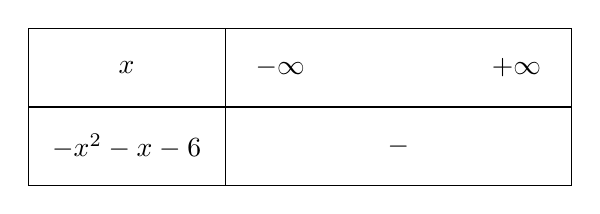
\begin{tikzpicture}
   \tkzTabInit[lgt = 2.5, espcl = 3, deltacl = 0.7]{$x$ / 1 , $-x^2 - x - 6$ / 1 }{$-\infty$, $+\infty$}
   \tkzTabLine{, - , }
\end{tikzpicture}

\end{center}

\begin{tcolorbox}[colback=yellow!20, colframe=black, sharp corners]
    \[
    \mathbf{S = \mathbb{R}}\quad\quad \textbf{1pt}
    \]
\end{tcolorbox}

    \item[(c)] \( 4x^2 - 4x + 1 \leq 0 \) 
    
\(
\textbf{Posons :} \quad 4x^2 - 4x + 1 = 0
\)

\(
\Delta = (-4)^2 - 4(4)(1) = 16 - 16 = 0
\)

\(
\text{Puisque } \Delta = 0, \text{ l'équation admet une unique solution :}
\)

\(
x = \frac{-(-4)}{2(4)} = \frac{4}{8} = \frac{1}{2}
\)

\begin{center}
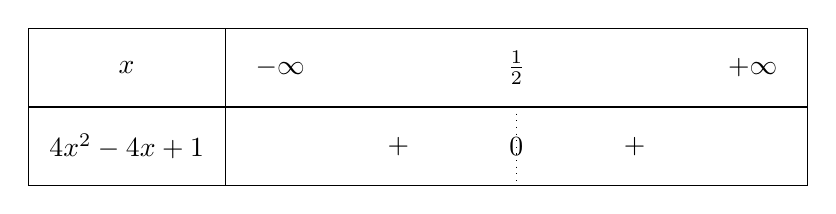
\begin{tikzpicture}
   \tkzTabInit[lgt = 2.5, espcl = 3, deltacl = 0.7]{$x$ / 1 , $4x^2 - 4x + 1$ / 1 }{$-\infty$, $\frac{1}{2}$, $+\infty$}
   \tkzTabLine{, + , z , + }
\end{tikzpicture}
\end{center}

\begin{tcolorbox}[colback=yellow!20, colframe=black, sharp corners]
    \[
    \mathbf{S = \emptyset}\quad\quad \textbf{1pt}
    \]
\end{tcolorbox}

\end{enumerate}
\section*{\underline{Exercice 5 :} 4.5pts}
\begin{enumerate}
    \item Factoriser les expressions suivantes :
 
\paragraph{•}   
\( A(x) = 25x^2 - 4 + (5x + 2)(x - 2) \)

\(
\begin{aligned}
A(x) &= 25x^2 - 4 + (5x + 2)(x - 2) \\
     &= (5x)^2 - 2^2 + (5x + 2)(x - 2) \\
     &= (5x - 2)(5x + 2) + (5x + 2)(x - 2) \\
     &= (5x + 2)\left[(5x - 2) + (x - 2)\right] \\
     &= (5x + 2)\left[6x - 4\right] \\
     &= 2(5x + 2)(3x - 2)
\end{aligned}
\)

\begin{tcolorbox}[colback=yellow!20, colframe=black, sharp corners]
    \[
    \mathbf{A(x) = 2(5x + 2)(3x - 2)}\quad\quad \textbf{0,75pt}
    \]
\end{tcolorbox}

\paragraph{•}
\(
C(x) = x^3 + 1 - 2x(x^2 - 1)
\)

\(
\begin{aligned}
C(x) &= x^3 + 1 - 2x(x^2 - 1) \\
     &= (x^3 + 1) - 2x(x^2 - 1)\\
     &=(x + 1)(x^2 - x + 1) - 2x(x - 1)(x + 1)\\
     &= (x + 1) \left[(x^2 - x + 1) - 2x(x - 1) \right]\\
     &= (x + 1) \left[x^2 - x + 1 - 2x^2 + 2x \right] \\
     &= (x + 1) \left[x^2 - 2x^2 - x + 2x + 1 \right] \\
     &= (x + 1) \left[-x^2 + x + 1 \right]
\end{aligned}
\)



\begin{tcolorbox}[colback=yellow!20, colframe=black, sharp corners]
    \[
    \mathbf{C(x) = (x + 1)(-x^2 + x + 1)}\quad\quad \textbf{0,75pt}
    \]
\end{tcolorbox}

\paragraph{•}   
\(
B(x) = x^3 - 8 + (x - 2)(2x - 3)
\)

\(
\begin{aligned}
B(x) &= x^3 - 8 + (x - 2)(2x - 3) \\
     &= x^3 - 2^3 + (x - 2)(2x - 3) \\
     &= (x - 2)(x^2 + 2x + 4) + (x - 2)(2x - 3) \\
     &= (x - 2) \left[(x^2 + 2x + 4) + (2x - 3) \right] \\
     &= (x - 2) \left[x^2 + 2x + 4 + 2x - 3 \right] \\
     &= (x - 2) \left[x^2 + 4x + 1 \right]
\end{aligned}
\)

\begin{tcolorbox}[colback=yellow!20, colframe=black, sharp corners]
    \[
    \mathbf{B(x) = (x - 2)(x^2 + 4x + 1)}\quad\quad \textbf{0,75pt}
    \]
\end{tcolorbox}
    
    \item Résolvons les équations et les inéquations suivantes :
    
    \( |4x + 3| = 2x + 1 \)

\(
\begin{aligned}
\textbf{Domaine de validité Dv:} & \quad 2x + 1 \geq 0 \Rightarrow x \geq -\frac{1}{2}
\end{aligned}
\)

\( Dv= \left[-\frac{1}{2};+\infty\right[ \)

\(
\begin{aligned}
|4x + 3| = 2x + 1 &\implies 4x + 3 = 2x + 1 \text{ ou } 4x + 3 = - (2x + 1) \\
                   &\implies 4x + 3 = 2x + 1 \text{ ou } 4x + 3 = -2x - 1 \\
                   &\implies 4x - 2x = 1 - 3 \text{ ou } 4x + 2x = -1 - 3 \\
                   &\implies 2x = -2 \text{ ou } 6x = -4 \\
                   &\implies x = -1 \text{ ou } x = -\frac{2}{3}
\end{aligned}
\)


\(
\begin{aligned}
x &= -\frac{2}{3}\notin \left[-\frac{1}{2};+\infty\right[ \quad \text{(Hors domaine, rejeté)}\\
x &= -1\notin \left[-\frac{1}{2};+\infty\right[ \quad \text{(Hors domaine, rejeté)}
\end{aligned}
\)

\begin{tcolorbox}[colback=yellow!20, colframe=black, sharp corners]
    \[
    \mathbf{S = \varnothing}\quad\quad \textbf{0,75pt}
    \]
\end{tcolorbox}

\( |-2x + 4| \leq 6 \)

\(
\begin{aligned}
|-2x + 4| \leq 6 &\implies -6 \leq -2x + 4 \leq 6\\
								 &\implies -6 - 4 \leq -2x + 4 - 4 \leq 6 - 4\\
								 &\implies -10 \leq -2x \leq 2 \\
								 &\implies -1 \leq x \leq 5
\end{aligned}
\)

\begin{tcolorbox}[colback=yellow!20, colframe=black, sharp corners]
    \[
    \mathbf{S = [-1, 5]}\quad\quad \textbf{0,75pt}
    \]
\end{tcolorbox}

\( |x - 2| = |7 - 3x| \)

\(
\begin{aligned}
|x - 2| = |7 - 3x| &\implies x - 2 = 7 - 3x \text{ ou } x - 2 = - (7 - 3x) \\
									 &\implies x - 2 = 7 - 3x \text{ ou } x - 2 = -7 + 3x \\
									 &\implies x + 3x = 7 + 2 \text{ ou } x - 3x = -7 + 2 \\
									 &\implies 4x = 9 \text{ ou } -2x = -5 \\
									 &\implies x = \frac{9}{4} \text{ ou } x = \frac{5}{2}
\end{aligned}
\)

\begin{tcolorbox}[colback=yellow!20, colframe=black, sharp corners]
    \[
    \mathbf{S = \left\{ \frac{9}{4}, \frac{5}{2} \right\}}\quad\quad \textbf{0,75pt}
    \]
\end{tcolorbox}

\bigskip

\(
\begin{aligned}
|7x - 2| \geq 2 &\implies 7x - 2 \geq 2 \text{ ou } 7x - 2 \leq -2 \\
                &\implies 7x \geq 2 + 2 \text{ ou } 7x \leq -2 + 2 \\
                &\implies 7x \geq 4 \text{ ou } 7x \leq 0 \\
                &\implies x \geq \frac{4}{7} \text{ ou } x \leq 0
\end{aligned}
\)
\begin{tcolorbox}[colback=yellow!20, colframe=black, sharp corners]
    \[
    \mathbf{S = \left] -\infty, 0 \right] \cup \left[ \frac{4}{7}, +\infty \right[}\quad\quad \textbf{0,75pt}
    \]
\end{tcolorbox}
\end{enumerate}

\section*{\underline{Exercice 6 :}2,25pts}

 Résolvons dans \( \mathbb{R} \times \mathbb{R} \) les systèmes d’équations suivants :
    
        \( S_1: 
        \begin{cases} 
            3x + 2y = 7 \\
            -4x + 5y = 6
        \end{cases} \)
        \quad ; \quad
        \( S_2: 
        \begin{cases} 
            -2x - y = 5 \\
            -8x + 7y = -13
        \end{cases} \)
        \quad ; \quad
        \( S_3: 
        \begin{cases} 
            x + y = 6 \\
            -3x - 17y = -18
        \end{cases} \)
        
\(
S_1:
\begin{cases} 
    3x + 2y = 7 \\
    -4x + 5y = 6
\end{cases}
\)

\(
\textbf{1. Élimination de \( x \) :} \quad 
\begin{cases} 
    4(3x + 2y) = 4(7) \\
    3(-4x + 5y) = 3(6)
\end{cases}
\)

\(
\begin{cases} 
    12x + 8y = 28 \\
    -12x + 15y = 18
\end{cases}
\)

\(
\text{On additionne :} \quad 12x + 8y - 12x + 15y = 28 + 18
\)

\(
23y = 46 \quad \Rightarrow \quad y = \frac{46}{23} = 2
\)

\(
\textbf{2. Calcul de \( x \) :} \quad \text{On remplace \( y = 2 \) dans \( 3x + 2y = 7 \)}
\)

\(
3x + 2(2) = 7 \quad \Rightarrow \quad 3x + 4 = 7
\)

\(
3x = 3 \quad \Rightarrow \quad x = 1
\)

\(
\textbf{Conclusion :} \quad S = \{ (1,2) \}
\)

\begin{tcolorbox}[colback=yellow!20, colframe=black, sharp corners]
    \[
    \mathbf{S = \{ (1,2) \}}\quad\quad \textbf{0,75pt}
    \]
\end{tcolorbox}

\(
S_2:
\begin{cases} 
    -2x - y = 5 \\
    -8x + 7y = -13
\end{cases}
\)

\(
\textbf{1. Élimination de \( x \) :} \quad 
\begin{cases} 
    4(-2x - y) = 4(5) \\
    -8x + 7y = -13
\end{cases}
\)

\(
\begin{cases} 
    -8x - 4y = 20 \\
    -8x + 7y = -13
\end{cases}
\)

\(
\text{On soustrait :} \quad (-8x - 4y) - (-8x + 7y) = 20 - (-13)
\)

\(
-11y = 33 \quad \Rightarrow \quad y = \frac{33}{-11} = -3
\)

\(
\textbf{2. Calcul de \( x \) :} \quad \text{On remplace \( y = -3 \) dans \( -2x - y = 5 \)}
\)

\(
-2x - (-3) = 5 \quad \Rightarrow \quad -2x + 3 = 5
\)

\(
-2x = 2 \quad \Rightarrow \quad x = -1
\)

\(
\textbf{Conclusion :} \quad S = \{ (-1, -3) \}
\)

\begin{tcolorbox}[colback=yellow!20, colframe=black, sharp corners]
    \[
    \mathbf{S = \{ (-1, -3) \}}\quad\quad \textbf{0,75pt}
    \]
\end{tcolorbox}

\[
S_3:
\begin{cases} 
    x + y = 6 \\
    -3x - 17y = -18
\end{cases}
\]

\(
\begin{aligned}
\textbf{1. Exprimer \( x \) en fonction de \( y \) :} \quad & x = 6 - y
\end{aligned}
\)

\(
\begin{aligned}
\textbf{2. Remplacement dans la deuxième équation :} \quad & -3(6 - y) - 17y = -18 \\
                                                           & -18 + 3y - 17y = -18 \\
                                                           & -14y = 0 \\
                                                           & y = 0
\end{aligned}
\)

\(
\begin{aligned}
\textbf{3. Calcul de \( x \) :} \quad & x = 6 - 0 = 6
\end{aligned}
\)

\(
\textbf{Conclusion :} \quad S = \{ (6, 0) \}
\)

\begin{tcolorbox}[colback=yellow!20, colframe=black, sharp corners]
    \[
    \mathbf{S = \{ (6, 0) \}}\quad\quad \textbf{0,75pt}
    \]
\end{tcolorbox}

\end{document}
